\section{Methodology}
Optimization of the nuclear fuel cycle is intended to develop 
a fuel cycle based on a specific objective or objectives. 
Optimization has previously been applied to the nuclear fuel 
cycle \cite{passerini_sensitivity_2012,andrianov_optimization_2019}
and other nuclear engineering \cite{chee_fluoride-salt-cooled_2022}.
This application of optimization uses \Cyclus \cite{huff_fundamental_2016}
to simulate the fuel cycle and Dakota \cite{adams_dakota_2019} to 
perform the optimization. In this chapter we demonstrate a methodology to 
apply this coupling to different optimization problems, and identify 
advantages and disadvantages of this methodology to optimize a nuclear 
fuel cycle. 

We developed three different optimization problems to apply to 
Scenarios 7 (no growth, once-through transition to the \gls{MMR}, Xe-100, 
and VOYGR) and 14 (no growth, limited recycling transition to the 
\gls{MMR}, Xe-100, and VOYGR): minimizing the \gls{SWU} capacity to 
produce \gls{HALEU}, minimizing the mass of \gls{SNF} for disposal, 
and minimizing both the \gls{HALEU} \gls{SWU} and the \gls{SNF} 
mass. To optimize these transitions, we consider six different 
variables: percent of \glspl{LWR} operating for 80 years (the \gls{LWR} 
lifetime), the build share 
of Xe-100s, the build share of \glspl{MMR}, the build share of VOYGRs, 
the discharge burnup of the Xe-100, and the discharge burnup of the 
\gls{MMR}. All of these variables were considered in the sensitivity 
analysis. The transition start time was also considered in the sensitivity 
analysis. However, that analysis showed that the transition start time has
a much smaller impact on each of the metrics and delaying the transition 
can lead to unfulfilled energy demand. Therefore, this parameter is 
not considered in the optimization of each scenario. 

For this work, the percent of \glspl{LWR} operating for 80 years 
was constrained to between 0-50\% of the current \gls{LWR} fleet. 
The build share of each advanced reactor was allowed to range between 
0-100\%, but the three parameters had to sum to 100\%. The discharge burnups 
are restricted to the values considered in the sensitivity analysis.

We coupled \Cyclus \cite{huff_fundamental_2016} with Dakota 
\cite{adams_dakota_2019} to perform this optimization. For the 
single-objective problems, we used the ``soga'' solve method in 
Dakota, which is a single-objective genetic algorithm. For the 
multi-objective problems we used the ``moga'' solve method in 
Dakota, which is a multi-objective genetic algorithm. Genetic algorithms
have previously been used to optimize fuel cycle transitions 
\cite{passerini_systematic_2014}, which led to the decision to use 
them for this work. Each of these methods have multiple 
hyperparameters that require careful tuning and selection. 

\subsection{Single-objective hyperparameter tuning}
Genetic algorithms have a variety of hyperparameters, such as the the 
population size, mutation rate, and crossover rate, that can affect 
the results of the algorithm. Therefore, we tuned multiple hyperparameters
to determine the best combination for this work and the exact algorithm 
used by Dakota. We performed the tuning by performing a grid search across 
the possible values for different parameters, a method recommended 
by Deb \cite{deb_multi-objective_2001} and demonstrated for reactor 
design optimization by Chee \cite{chee_fluoride-salt-cooled_2022}. 
Not all hyperparameters or all possible values of the hyperparameters 
were considered. We downselected from 
the possible hyperparameters and values defined in the Dakota Reference 
Manual based on hyperparameters defined in previous generic algorithms 
for nuclear energy applications
\cite{passerini_systematic_2014,chee_fluoride-salt-cooled_2022},
personal intuition, and limitations on time to perform 
the tuning.

The 
first grid search performed 40 iterations of different hyperparameter 
values across a coarse grid. The total number of samples was restricted to 
300 for each evaluation, which restricts the population size and the 
number of generations, as the product of these two must equal the 
total number of samples. Table \ref{tab:soga_tuning} describes 
the hyperparameters considered in the tuning and the range of possible 
values considered. Some of the variables, such as the mutation 
type, take discrete values while others, such as the crossover 
rate, can take continuous values. The crossover rate, mutation 
rate, and constraint penalty were treated as continuous for this 
tuning, and therefore were randomly sampled within the defined range. 
The population size can be a continuous variable, but was 
treated as discrete for this initial search to provide a well-defined 
number of generations. Hyperparameters not varied in the tuning, and 
help constant for all runs include the convergence type (kept at
``best fitness tracker'' ), the fitness type (kept at ``merit function''),
and the random seed (kept at the same value for all runs).

\begin{table}
    \centering 
    \caption{Hyperparameters and values considered in tuning. If a range 
    of values is provided, then the hyperparameter a random value in 
    that range was selected.}
    \label{tab:soga_tuning}
    \begin{tabular}{c c c}
        \hline
        Hyperparameter & Coarse Search & Fine Search \\
        \hline 
        Experiments [\#] & 1-40 & 41-60 \\
        Population size [\#] & 5, 10, 25, 50, 100 & 25, 50\\
        Constraint penalty & 0.5 $\leq$ x $\leq$ 2 & 1 $\leq$ x $\leq$ 2\\
        Crossover rate & 0.1 $\leq$ x $\leq$ 0.9 & 0.3 $\leq$ x $\leq$ 0.9\\
        Mutation type & replace uniform, offset normal & replace uniform, offset normal\\
        Mutation rate & 0.01 $\leq$ x $\leq$ 0.2 & 0.025 $\leq$ x $\leq$ 0.19\\
        \hline       
    \end{tabular}
\end{table}


Figure \ref{fig:soga_coarse_tuning} shows the results of the coarse tuning 
for the single objective problem. From these results, we observe that the 
\gls{HALEU} \gls{SWU} capacity tends to be lower with:
\begin{itemize}
    \item a population size between 10 and 50
    \item an ``offset normal'' mutation type
\end{itemize}

\begin{figure}
    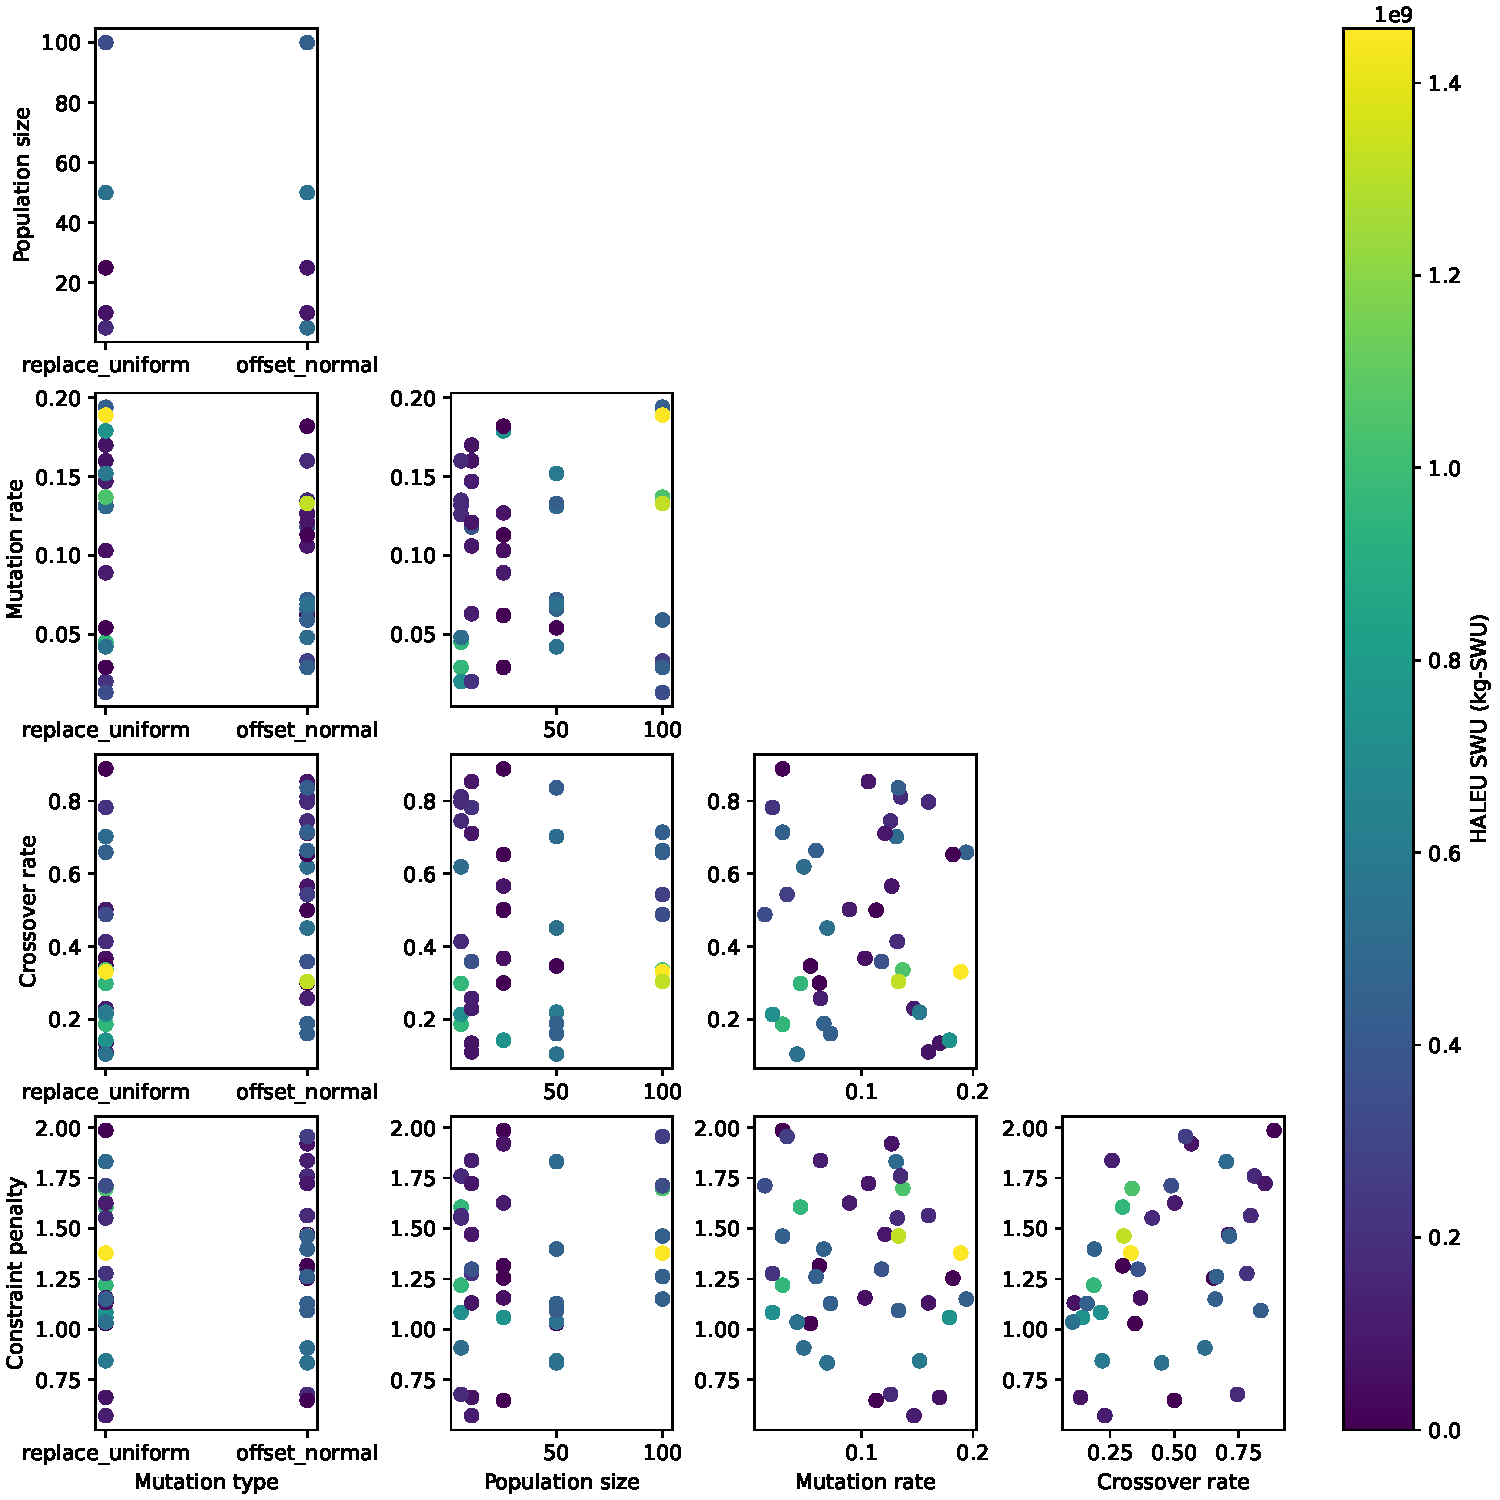
\includegraphics[scale=0.7]{soga_coarse_tunng.pdf}
    \caption{Results of coarse tuning for the single-objective 
    optimization.}
    \label{fig:soga_coarse_tuning}
\end{figure}

Five of the tuning runs reached the theoretical minimum for \gls{HALEU} \gls{SWU} 
capacity of 0 kg-SWU, which occurs when only the VOYGR is deployed. Four of the 
runs had a population size of 25 and one had a population size of 50. Three of 
them used an ``offset normal'' mutation 
type, while two used a ``replace uniform'' mutation type. The smallest mutation 
rate was 0.029 and the largest is 0.182, so this hyperparameter spans most of 
the space. The crossover rates ranges between 0.3-0.888. The constraint 
penalty ranges between 0.648-1.986, with four of the five runs having constraint 
penalties above 1.0. Based on this information, we ran another 20 tuning runs with 
a finer grid for some of the parameters, defined in the ``Fine Search'' column of 
Table \ref{tab:soga_tuning}, based on these results. 

Three of the fine tuning cases found the theoretical minimum. Observations about 
these cases include:
\begin{itemize}
    \item All had a population size of 25
    \item The mutation rates varied between 0.123-0.168
    \item The crossover rates varied between 0.415-0.70, with two of the three 
          runs having crossover rates between 0.4-0.5
    \item The constraint penalty values ranged between 1.157-1.792
\end{itemize}
Combined with the observations from the coarse tuning, the hyperparameter 
tuning suggests that a population size of 25, a mutation rate above 
0.1, crossover rate between 0.4-0.7, and a constraint penalty 
between 1.1-1.6 should be used. For the mutation type, the replace uniform 
method and the offset normal methods resulted in four and five runs that 
reached the theoretical minimum, respectively, across the two sets of 
tuning cases. As a whole, this hyperparameter did not cause as much of 
an effect on the results.

In addition to hyperparameters, another consideration in the tuning process 
is how well the linear constraint of the problem (all of the advanced 
reactor build shares sum to 100) is met. According to the Dakota 
Reference Manual page for the ``SOGA'' optimization method, this 
optimization method does not always strictly adhere to any linear 
constraints defined by the user \cite{adams_dakota_2019}. In practice, 
this means that the constraint will not be met by every evaluation but the 
final solution will meet the constraint. Because not all evaluations 
adhere to the constraint, this method is likely to take more time and 
compute resources than the optimization methods in Dakota that will 
adhere to the constraint on every evaluation. 

The build share for the \gls{MMR} and Xe-100 are each under 1\% for all of 
the tuning runs that reached the theoretical minimum. While these values 
are not zero, the workflow applied rounded down these values to zero, which 
resulted in none of these reactors being deployed and reaching the 
theoretical minimum for \gls{HALEU} {SWU}. The rounding of the build share 
values (which is also applied to the other input parameters) leads to an 
undersupply of power in all scenarios, because the largest VOYGR build 
share is 99\%. The undersupply of power demonstrates that fuel cycle 
modelers need to have a strong understanding of their assumptions, such 
as how numbers are rounded, when using the methodology for optimizing a 
fuel cycle. 

\subsubsection{Hyperparameter selection}
Based on the tuning performed, we selected values for each of the 
hyperparameters. Table \ref{tab:soga_parameters} defines the 
parameters used with the single-objective optimization schemes. These 
hyperparameters match the hyperparameter values of tuning run 29, 
which resulted in a \gls{HALEU} \gls{SWU} value of 0. These hyperparameters 
were selected over the hyperparameters of the other runs that resulted in 
0 \gls{HALEU} \gls{SWU} because this run selected variables that came closest to 
meeting the constraint of a 100\% advanced reactor build share after the rounding 
was applied. We applied these hyperparameters to all single-objective 
optimization problems in this work. 

\begin{table}
    \centering
    \caption{Hyperparameters selcted for single-objective optimization.}
    \label{tab:soga_parameters}
    \begin{tabular}{c c}
        \hline
        Parameter & Value \\
        \hline
        Population & 25 \\
        Constraint penalty & 1.554\\
        Crossover rate & 0.753\\
        Mutation type & offset normal\\
        Mutation rate & 0.045\\
        \hline
    \end{tabular}
\end{table}

\subsection{Multi-objective hyperparamter tuning}
Hyperparameter tuning for a multi-objective problem is more complicated 
than tuning for a single-objective problem. In multi-objective 
problems, there is no single best solution but rather many solutions 
that form a Pareto front \cite{adams_dakota_2019}. The points on a 
Pareto front indicate that further improvement of one objective 
results in a worsening of another objective. Therefore, to tune the 
hyperparameters of a multi-objective problem, one tunes base on the 
hypervolume of the Pareto front \textbf{Find citation}. The 
hypervolume of a Pareto front is calculated by calculating the area 
contained by 

Used equal weights for each objective. 

\subsubsection{Hyperparameter selection}

\section{Once-through optimization}
\subsection{Minimize HALEU SWU}
By applying the hyperparameters to an optimization problem to minimize the 
\gls{HALEU} \gls{SWU} capacity needed by this transition scenario, Dakota
found a minimum with the values defined in Table \ref{tab:soga_ot_haleu}.

\begin{table}
    \centering 
    \caption{Values resulting in a minimum \gls{HALEU} \gls{SWU} capacity for 
              a once-through transition scenario.}
    \label{tab:soga_ot_haleu}
    \begin{tabular}{c c}
        \hline
        Variable & Value \\
        \hline
        LWR Lifetime & \\
        Xe-100 build share & \\
        MMR build share & \\
        VOYGR build share & \\
        Xe-100 burnup & \\
        MMR burnup & \\
        \hline
    \end{tabular}
\end{table}

\subsection{Minimize waste mass}
By applying the hyperparameters to an optimization problem to minimize the 
\gls{HALEU} \gls{SWU} capacity needed by this transition scenario, Dakota
found a minimum with the values defined in Table \ref{tab:soga_ot_waste}.
The minimum waste mass determined through the optimization is 22,703 MT. 

\begin{table}
    \centering 
    \caption{Values resulting in a minimum \gls{HALEU} \gls{SWU} capacity for 
              a once-through transition scenario.}
    \label{tab:soga_ot_waste}
    \begin{tabular}{c c}
        \hline
        Variable & Value \\
        \hline
        LWR Lifetime & 49.31\%\\
        Xe-100 build share & 85.93\%\\
        MMR build share & 6.53\%\\
        VOYGR build share & 9.31\%\\
        Xe-100 burnup & 185 MWd/kgU\\
        MMR burnup & 90 MWd/kgU\\
        \hline
    \end{tabular}
\end{table}

Each of the variables either match or trend towards expectations for this problem. 
Based on the transition analysis (Chapter \ref{ch:once_through_results}) and 
sensitivity analysis (Chapter \ref{ch:sa}), one would expect that to minimize 
the spent fuel mass the \gls{LWR} lifetime percent, Xe-100 build share, 
Xe-100 burnup, and \gls{MMR} burnup would all be maximized while the \gls{MMR} 
and VOYGR build shares are minimized with the deployment of \glspl{MMR} favored 
over VOYGR deployment. The Xe-100 and \gls{MMR} burnup values are at the maximum 
values considered for this work, which matches expectations. The \gls{LWR} lifetime 
extension percent is near the maximum considered for this work, which suggests that 
the waste mass from advanced reactors could be further decreased by using the 
maximum of this input parameter. 

The advanced reactor build shares trend towards expectations, but don't fully 
meet them. The deployment of Xe-100s over the other advanced reactors is consistent 
with the results in Table \ref{tab:nogrowth_waste}, which shows that only deploying 
Xe-100s results in less spent fuel mass than the other combinations of the reactors. 
Therefore, one would expect that the Xe-100 build share would be 100\%. Then combined 
with the other input parameters (the \gls{LWR} lifetime percent and Xe-100 burnup 
specifically) the optimized transition scenario would result in less spent fuel 
mass than the scenarios considered in Chapter \ref{tab:nogrowth_waste}.

\subsection{Minimize HALEU SWU and waste mass}

\section{Recycling optimization}
\subsection{Minimize HALEU SWU}

\subsection{Minimize waste mass}

\subsection{Minimize HALEU SWU and waste mass}
